\documentclass[12pt]{article}

\usepackage[utf8]{inputenc}
\usepackage{geometry}
\geometry{a4paper, total={170mm,257mm}, left=20mm, top=20mm, }
\usepackage{graphicx}
\usepackage{titling}
\usepackage{lipsum}  
\usepackage{cmbright}
\usepackage[utf8]{inputenc}
\usepackage{graphicx}
\usepackage[T1]{fontenc}
\usepackage[french]{babel}
\usepackage[document]{ragged2e}
\usepackage{geometry}
\usepackage{fancyhdr}
\usepackage{tabularx}
\usepackage{fancyvrb}
\usepackage{cite}
\usepackage{subfig}
\usepackage{enumitem}
\usepackage{hyperref}
\usepackage{amsmath}
\usepackage{floatrow}
\usepackage{subfiles}
\usepackage{titlesec}
\usepackage[table,xcdraw]{xcolor}
\usepackage{booktabs}
\usepackage{pdfpages}
\usepackage{afterpage}
\usepackage{pifont}
\usepackage{systeme}
\usepackage{url}
\usepackage{csquotes}
\usepackage{courier}

% ------------------------------------------------------------------------------

\begin{document}

    \begin{LARGE}
        \textbf{Charte Graphique}
    \end{LARGE}

    \vskip 0.5 cm

    \begin{large}
        \textbf{Palette de couleur}
    \end{large}

    \vskip 0.25 cm
    
    Afin de créer un site dont le visuel était à la fois plaisant et intuitif, il était important de choisir des couleurs qui permettaient d'avoir un contraste élevé, même en niveau de gris, mais aussi agréables, tout en rappelant l'utilité du site.\\
    Pour cela, plusieurs chartes graphiques ont été proposées, et votées au sein de l'équipe.
    
    \vskip 0.2 cm
    
    La palette de couleur choisie a été renommée "Vert pomme", et elle est donc constituée des couleurs qui seront principalement retrouvées sur le site.

    \begin{figure}[h!]
        \centering
        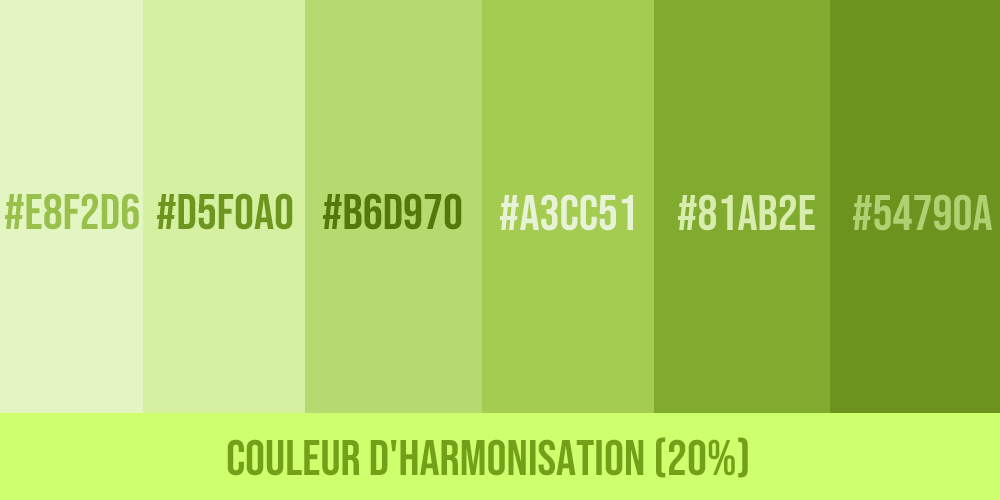
\includegraphics[scale = 0.45]{static/Pomme Palette 1.png}
        \small{\emph{Palette Pomme}}
        \label{fig:Palette}
    \end{figure}

    Comme dit précédemment, cette palette a été également conçue afin d'être assez contrastée dans le cas d'un daltonisme : ainsi, bien que cette palette soit composée de couleurs dans des tons verts, le contraste entre les nuances soit suffisant pour distinguer les écritures du fond.
    
    \begin{figure}[h!]
        \centering
        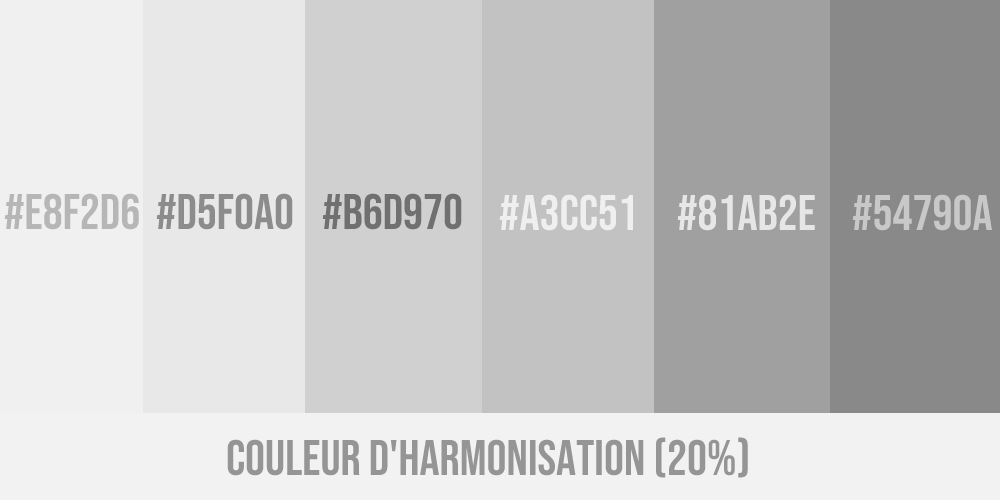
\includegraphics[scale = 0.45]{static/greypal.png}
        \small{\emph{Palette Pomme en niveau de gris}}
        \label{fig:Palette2}
    \end{figure}

% ------------------------------------------------------------------------------

    \newpage

% ------------------------------------------------------------------------------

    \begin{large}
        \textbf{Logo du site}
    \end{large}

    \vskip 0.25 cm

    Une fois la palette de couleur établie, nous nous sommes penchés sur la question du nom, et du logo pour notre site. Après plusieurs minutes de réflexions, nous avons fini par choisir le nom de TELEPOMME d'ici. Un rappel phonique à cette école qui est à la naissance du projet, tout en étant un écho à notre palette nouvellement choisie. Puis, finalement, le logo se présenta presque comme une évidence.

    \begin{figure}[h!]
        \centering
        
\includegraphics[scale = 0.12]{static/Logo TELEPOMME d'ici.png}
        \small{\emph{Logo de TELEPOMME d'ici}}
        \label{fig:Logo}
    \end{figure}

    Quelques tests avec un visuel du site fait sur un logiciel de dessin a permis d'assurer une harmonisation du logiciel avec le reste de la charte graphique.

    \begin{figure}[h!]
        \centering
        
\includegraphics[scale = 0.12]{static/0 - Barre exemple.png}
        \small{\emph{Exemple d'une partie du site}}
        \label{fig:Ex_site}
    \end{figure}

% ------------------------------------------------------------------------------

    \newpage

% ------------------------------------------------------------------------------

    \begin{large}
        \textbf{Icones de fruits et légumes}
    \end{large}

    \vskip 0.25 cm

    Lors de la réunion du 10/12/2022, alors que nous parlions de l'égalité entre les différents vendeurs de la plateforme, il a été décidé que les images de fruits, légumes et autres produits, seraient remplacés par des icones.\\
    Ainsi, plusieurs propositions d'icones ont été posées, différant par leur style et leur couleurs, jusqu'à ce que soit choisie la forme finale.

    \begin{figure}[h!]
        \centering
        
\includegraphics[scale = 0.17]{static/Pomme.png}
        \hspace{2 cm}
        
\includegraphics[scale = 0.17]{static/Tomate.png}\\
        \small{\emph{Icone de la pomme}}
        \hspace{5 cm}
        \small{\emph{Icone de la tomate}}
        \label{fig:Icones}
    \end{figure}

    Enfin, il a été décidé que comme il n'était pas impossible qu'une icone soit manquante, des icones par défaut seraient créées. 

    \vskip 0.2 cm

    \begin{figure}[h!]
        \centering
        
\includegraphics[scale = 0.2]{static/Base_Fruit.png}\\
        \small{\emph{Icone de fruit par défaut}}
        \label{fig:fruit_default}
    \end{figure}    

\end{document}
